\chapter{Extracción de información}

Utilizando nuestra página web se van a poder obtener distintas muestras de Córdoba y Buenos Aires. Pero ¿ cómo podemos analizar estos audios correctamente?. Un archivo wav, como los que captura la página cada una de las pruebas, posee muchísima información. Es por esto que debemos seleccionar correctamente qué partes de la información nos sirve y qué partes podemos descartar. 

\section{Alineación forzada}

Una grabación de una frase posee muchísima información. Debemos seleccionar que parte de esta grabación nos interesa y que parte puede ser descartada. Para ello etiquetamos en la duración del audio en que partes se pronunció cada fonema y también cada palabra. Por ejemplo: si tenemos la grabación de la frase `El canapé salió espectacular’ vamos a tener un archivo aparte que básicamente nos dice \textit{`espectacular se escucha entre el minuto 0.90 y 1.18’}. Lo mismo sucede para cada fonema de la grabación.

Un dato muy importante es que este etiquetado idealmente no debe tener que ser realizado con intervención de un humano. Ya que, si tenemos muchos audios tendríamos que hacerlo uno por uno y sería un trabajo muy arduo. De esto se encarga la alineación forzada. Las partes que debemos extraer de los audios son las partes donde se encuentran la diferencias de cada regla descripta anteriormente. Debemos tener una herramienta que nos permita obtener esos pequeños fragmentos de audio para analizar sus diferencias. 

\subsection{Prosodylab Aligner}

%If you use this tool, we would appreciate it if you cite the following paper:
%Gorman, Kyle, Jonathan Howell & Michael Wagner (2011). Prosodylab-Aligner: A tool for forced alignment of laboratory speech. Proceedings of Acoustics Week in Canada, Quebec City.

Luego de buscar bastante encontramos con una herramienta llamada ProsodyLab Aligner \cite{prosodylab}. Su función es realizar alineaciones automáticas en cada uno de los audios de forma fácil. O sea, va analizar cada audio y mediante un diccionario determina en que momento se dijo cada fonema. El formato utilizado para devolver estas marcas es TextGrid. El problema de la alineación es un caso particular de la alineación automática.

Algo en que se destaca esta herramienta es que no necesita datos de entrenamiento. Sólo con una hora de grabación es suficiente para correrlo y obtener resultados. Otra ventaja es que puede utilizarse para cualquier idioma. Esta herramienta esta hecha íntegramente en lenguaje Python (versión 2.5) y scripts de Linux. Utiliza fuertemente HTK que es una librería para utilizar Modelos Ocultos de Markov fácilmente y SoX que nos permite trabajar con audio a través de la consola. Los Modelos Ocultos de Markov \cite{rabiner} (en ingles HMM) básicamente tratan de predecir qué fonemas aparecen en cada parte de los audios utilizando las diferentes muestras y la lista de fonemas pronunciada en cada grabación. Por ejemplo: mediante este modelo matemático el programa analiza en cuales grabaciones de la misma frase se produce un mismo fonema. Ese fonema va a ser marcado de igual forma en el TextGrid de cada grabacion.

Los requisitos para utilizar esta herramienta son: una hora de grabación y un diccionario fonético que nos provea para cada palabra los distintos fonemas que la componen. La hora de grabación la debíamos cumplir recolectando grabaciones de la página web. Esta meta era posible de realizar. La creación de un diccionario fonético era más complicado, ya que debía ser en español. Gracias a \textit{Laboratorio de Investigaciones Sensoriales} que nos prestó su diccionario pudimos utilizar esta herramienta. Un diccionario fonético es básicamente un listado con las palabras que utilizamos y su división en fonemas. Es importante esto ya que va a ser usado por el alineador para describir los fonemas de cada palabra en cada frase.

\section{Extracción de atributos}

La extracción de datos fue realizado utilizando el lenguaje Python. Elegimos ese ya que es un lenguaje de fácil de programar y tiene muchas librerías útiles para este tipo de casos. Utilizamos una muy conocida llamada Numpy versión 1.6.1. Esta librería se utiliza para realizar cálculos matemáticos de precisión. Nosotros la utilizamos para tener buena precisión en el cálculo de cada uno de los atributos.

El primer paso antes de extraer atributos es alinear con el ProsodyLab Aligner. Este al finalizar una alineación nos devuelve un archivo donde se encuentra como fueron realizadas esas alineaciones. Este archivo se llama `.SCORES’ y en el se encuentra una lista de todos los audios seguidos de un valor. Este valor nos permite ver la verosimilitud de las alineaciones. Si una alineación fue similar a otra va a tener aproximadamente un valor similar. En cambio, si posee una alineación muy distinta va a tener valores muy distintos. Este va a ser el primer filtro para el extractor. Ordenando los audios en esta escala notamos que los menores poseen alineaciones malas, entonces definimos un umbral para el cual aceptar y rechazar la alineación. Si bien este procedimiento es efectivo, notamos que se encuentran algunos falsos positivos, o sea archivos que tienen un buen punto de score pero la alineación es mala. Al tener pocas grabaciones no pudimos aceptar estos casos, debimos corregirlos uno por uno.

Después de la alineación realizada se ejecuta el extractor de atributos. Este posee como input los archivos Wav y los archivos TextGrid que corresponden a las alineaciones temporales de cada fonema en cada audio. El workflow del extractor se puede ver en \ref{workflow}). 

El main principal del programa va a tomar de a uno las grabaciones y va a aplicarle un conjunto de funciones. Cada una de estas funciones van a calcular un atributo. Los atributos se pueden dividir en dos tipos: uno correspondiente a atributos temporales o calculados solamente en el TextGrid y otro a atributos acústicos utilizando no sólo el TextGrid sino el calculo de MFCC que veremos más adelante. Si el atributo esta presente en la grabación tendremos ese dato en la extracción, sino se dejará como nulo. Luego juntamos todos los resultados de estas grabaciones y generamos el archivo Arff. El archivo Arff básicamente tiene por cada linea una grabación y  seguido todos los resultados del calculo de los atributos separado por comas. 

\begin{figure}[h!]
    \centerline{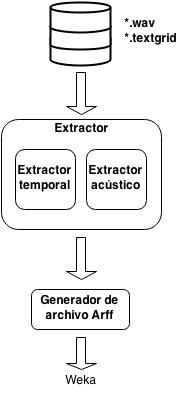
\includegraphics[width=0.5\textwidth]{diagrama_workflow} }
    \caption{Diagrama workflow}
    \label{workflow}
\end{figure}

Veamos cada uno de los dos tipos de atributos:

\subsection{Atributos temporales}

Los atributos temporales corresponden a los atributos de duración de los fonemas y la sílabas de cada frase. Para calcularlos utilizamos como input el TextGrid generado en la alineación. Básicamente estas funciones recorren el TextGrid buscando un patrón en particular y lo miden.

Las mediciones son normalizadas de dos formas: primero una normalización utilizando:

\hspace{2cm} \[\frac{ \bar{X} - \mu }{ \sigma }\]

y luego otra asumiendo que $\mu = 0$. 

\hspace{2cm} \[\frac{ \bar{X} }{ \sigma }\]

Esta ultima tiene el nombre de half normal distribution.

%todo: agregar imagen explicando normalización

Los atributos temporales se dividen en dos grupos: fonéticos y silábicos. Cada grupo calcula de la misma forma la normalización pero uno va a tener en cuenta fonemas y otro sílabas. Veamos cuales son:

\subsubsection{Atributos fonéticos}

\begin{itemize}
    \item \textbf{Duración de la `kt’:} este atributo vamos a buscar el patrón /kt/ en los TextGrids y luego a medir la duración del fonema /k/ en ese intervalo. Este atributo intenta medir la diferencia explicada en la regla 4 que nos indica medir dicho fonema.
    \item \textbf{Duración de la `sc’:} ídem con /sc/ y midiendo el fonema /s/. Este corresponde a la regla 3 que referencia a la duración del fonema /s/ anterior a /c/.  
    \item \textbf{Duración de la `ll’:} buscamos el patrón /ll/ y lo medimos. Este atributo hace referencia a la regla 5 que mide dicho fonema.
    \item \textbf{Duración de la `rr’:} ídem para /r/ fuerte. Referencia a la regla 6 que hace hincapié en este fonema.
    \item \textbf{Duración de la `s’ final:} ídem para las /s/ de final de palabra. Corresponde a la regla 2 que hace referencia a la aspiración de la /s/ de final de las palabras.  
    \item \textbf{Duración de cada fonema:} este atributo mide la cantidad de fonemas y realiza un promedio. Este no se realiza normalización.  
    \item \textbf{Duración de cada vocal:} contabilizamos cada vocal y luego realizamos su normalización utilizando la duración de cada fonema.
    \item \textbf{Duración de cada consonante:} ídem anterior para consonantes. 
\end{itemize}

El cálculo de un atributo fonético se realiza de la siguiente forma: supongamos que queremos calcular la duración de la `kt’. Los valores de la normalización serán: para $\mu$ se calculará como el promedio de duración de los fonemas en la frase en cuestión. Para $\sigma$ será el desvío estándar de la duración de los fonemas de la frase. Y para $\bar{X}$ será el promedio de duración de los fonemas de la forma /k/ en el intervalo /kt/. Ídem para los demás atributos.

En definitiva se busca el patrón definido por el atributo, se mide la cantidad de ocurrencias que posee y luego se realiza su normalización de las dos formas utilizando esos valores. 

\subsubsection{Atributos silábicos}

Vamos a hacer un análisis de la sílabas. Los atributos que usamos son:

\begin{itemize}
    \item \textbf{Duración de la sílaba acentuada:} en cada una de las frases vamos a buscar la sílaba acentuada de cada palabra, mediremos su duración y normalizaremos con las demás sílabas.
    \item \textbf{Duración de la sílaba anterior a la acentuada:} realizamos el mismo calculo anterior pero con la sílaba previa a la acentuada. 
\end{itemize}

El cálculo de un atributo silábico se realiza tomando estos valores: tomando como atributo la duración de la sílaba acentuada $\mu$ representará el promedio de duración de sílabas en la frase. $\sigma$ será el desvío estándar de la duración de las sílabas en la frase. Y finalmente $\bar{X}$ será el promedio de duración de las sílabas acentuadas en la frase. Para cada uno de estos valores se calcula los dos tipos de normalización.

Estos atributos usamos para poder medir fuertemente la Regla 1, que esta es la más resaltada de la tonada cordobesa. Para saber cual es la sílaba acentuada se realizó un script que describe para cada frase cuales son sus sílabas acentuadas. Este se encuentra en el Apéndice.

\subsection{Atributos acústicos}

Los atributos acústicos utilizan las propiedades de los wavs grabados. Para ello debimos extraer información con algún método que permita medirlos. Elegimos el calculo de MFCC ya que tiene relación directa con la percepción auditiva humana. 

\subsubsection{Mel Frequency Cepstral Coefficients}

%http://practicalcryptography.com/miscellaneous/machine-learning/guide-mel-frequency-cepstral-coefficients-mfccs/

La forma en que hablamos se produce por varias articulaciones. Algunas de ellas pueden ser: dientes, lengua, traquea etc. Estas articulaciones trabajan de forma tal para producir el sonido. Pero también funcionan para darle forma y aplicarle un filtro al sonido producido. Si sabemos correctamente que filtro se le aplica, podremos saber que sonido produce. La forma y el filtro asociado nos muestra donde esta la fuerza en el fonema. Este filtro es muy importante para entender la percepción humana.

Las señales de audio poseen muchas variaciones continuamente. En periodos cortos de tiempo estas variaciones se reducen. Vamos a dividir todo el audio en pequeños frames para calcular en ellos los coeficientes. El tamaño de cada frame esta entre 20-40 ms. Si la variación es menor a este frame, habrá pocas pruebas para tenerla en cuenta y entonces la descartaremos.

Luego para cada frame se calcula el espectro de frecuencia. Esto se viene motivado por un órgano que se encuentra en la oreja llamado Cóclea. Este vibra de diferente forma al llegarle cada frecuencia del sonido. Al vibrar, activa nervios que representan las distintas frecuencias que escuchamos. Dividir el sonido en períodos intenta mostrar que frecuencias están activas.

La Cóclea no reconoce diferencias entre dos frecuencias muy cercanas. Esto se incrementa mientras más alejada esta esa frecuencia. Para representar esta idea se utiliza un filtrado por escala de Mel. Esta escala es una aproximación de nuestra percepción. A frecuencias menores a los 1 Khz el filtro se comporta de forma lineal. A partir de ese valor, se comporta de forma logarítmica. 

%http://i.stack.imgur.com/YUH48.gif

% todo: Aca se introduce los filtros onda serrucho. 
Mientras mas aumentamos la frecuencia, mas anchos son los filtros aplicados. Por ejemplo, ya en 4 Khz se aplican 20 filtros. Lo importante es ver cuanta energía hay en las frecuencias involucradas en el filtro. Luego que tenemos la energía de estos tramos le aplicamos la función logaritmo. De esta forma, para valores grandes de frecuencias su valor se decrementarán y no será igual que las pequeñas que poseen forma lineal. Esto se ajunta mejor a como escucha el oído. Para finalizar se computa DCT de las energías filtradas. 

El siguiente pseudocódigo explica paso a paso como se calcula los coeficientes:
\lstset{ %
language=C++,                % choose the language of the code
basicstyle=\footnotesize,       % the size of the fonts that are used for the code
numbers=left,                   % where to put the line-numbers
numberstyle=\footnotesize,      % the size of the fonts that are used for the line-numbers
stepnumber=1,                   % the step between two line-numbers. If it is 1 each line will be numbered
numbersep=5pt,                  % how far the line-numbers are from the code
backgroundcolor=\color{white},  % choose the background color. You must add \usepackage{color}
showspaces=false,               % show spaces adding particular underscores
showstringspaces=false,         % underline spaces within strings
showtabs=false,                 % show tabs within strings adding particular underscores
frame=single,           % adds a frame around the code
tabsize=2,          % sets default tabsize to 2 spaces
captionpos=b,           % sets the caption-position to bottom
breaklines=true,        % sets automatic line breaking
breakatwhitespace=false,    % sets if automatic breaks should only happen at whitespace
escapeinside={\%*}{*)}          % if you want to add a comment within your code
}
\begin{lstlisting}
MFCC (Mel frequency cepstral coefficient):
1) Aplicar la derivada de Fourier de la se\~nal. -> Espectro
2) Mapear las amplitudes del espectro a la escala mel.
3) Calcular el logaritmo.
4) Aplicar la transformada de coseno discreta (DCT).
5) Los MFCC son las amplitudes del espectro resultante.
\end{lstlisting}

Este algoritmo se calcula para un segmento del audio. El audio se debe dividir en frames de 20 o 30 milisegundos pero avanzando 10 o 15 milisegundos. Hay superposiciones en cada segmento. Al finalizar el algoritmo obtenemos 13 atributos acústicos de ese segmento. Podemos realizar la derivada de estos atributos y la segunda derivada para obtener más atributos. Estos atributos corresponden a el estiramiento de los fonemas a través del tiempo. En total derivando dos veces llegan a 33 atributos acústicos.

Debemos extraer datos de los wavs grabados. Para ello debemos analizarlos y que ese análisis nos de una medida que pueda compararse. El análisis debe tener en cuenta como lo percibe un humano. Las frecuencias de Mel ayudan a describir la percepción humana del lado de las frecuencias que escucha. 

\subsubsection{Implementación}

Para realizar el calculo de estos coeficientes se utilizó un script en Matlab. El creador del script es Kamil Wojcicki y utiliza los 33 atributos utilizando sus primeras y segundas derivadas. El extractor necesita estos valores para cada audio a extraer. Es por eso que se conecta con Matlab a través de un wrapper para calcular el script y luego continuar con la extracción.

\subsection{Nomenclatura utilizada}
Para referenciar cada una de los atributos debimos definir una nomenclatura. La definición que tomamos es la siguiente:
\begin{center}
\textit{TIPO+``\_''+ATRIBUTO+``\_''+NORMALIZACIÓN} 
\end{center}
donde:
\begin{itemize}
  \item \emph{TIPO} puede ser \emph{FON, SIL o ACU}. Esto corresponde al tipo de atributo, si es fonético, silábico o acústico.
  \item \emph{ATRIBUTO} puede ser \emph{kt, ll, sc, rr, Sfinal, vowel o consonant} haciendo alusión a cada una de los atributos. También aquí se encuentran los atributos generados por MFCC cuyos nombres son de la forma \emph{(Min $|$ Max $|$ Avg) + (KT $|$ LL $|$ SC $|$ RR)}. Parahacer referencia a las reglas sobre atributos silábicos utilizamos los nombres de \emph{syllableAccent} y \emph{prevSyllableAccent} para la duración de la silaba acentuada y su anterior.
  \item \emph{NORMALIZACIÓN} corresponde al tipo de normalización realizada. Estas pueden ser \emph{norm} haciendo alusión a normalización o \emph{normhd} haciendo alusión a normalización tomando $mu=0$.
\end{itemize}
 
Por ejemplo: definimos SIL\_prevSyllableAccent\_normhd como la duración de la silaba anterior a la acentuada aplicando normalización con $mu=0$. Todos los nombres y a que atributo se refieren se puede ver en el apéndice de atributos.

A continuación veamos el análisis que realizamos utilizando todos estos atributos.